\documentclass[10pt]{article}

% =============================================================================
% DATOS GENERALES DEL TRABAJO
% =============================================================================
\newcommand{\materia}{Instrumentación Biomédica I}
\newcommand{\institucion}{Instituto Tecnológico de Buenos Aires}
\newcommand{\numeroTP}{4}
\newcommand{\nombreTP}{Oximetría SpO2}
\newcommand{\anioTP}{2026}

% =============================================================================
% FORMATO EXIGIDO POR LA CÁTEDRA
% =============================================================================
\textheight=21cm
\textwidth=15cm
\topmargin=-0.5cm
\oddsidemargin=1cm
\evensidemargin=1cm
\parindent=0mm

% =============================================================================
% PAQUETES
% =============================================================================

% Codificación e idioma
\usepackage[utf8]{inputenc}
\usepackage[T1]{fontenc}
\usepackage[spanish,es-tabla]{babel}

% Matemática y unidades
\usepackage{amsmath,amssymb}
\usepackage{siunitx}
\sisetup{output-decimal-marker={,}}

% Figuras y tablas
\usepackage{graphicx}
\graphicspath{{imagenes/}}
\DeclareGraphicsExtensions{.pdf,.png,.jpg,.jpeg}
\usepackage{float}
\usepackage{subcaption}
\usepackage{booktabs}
\usepackage{array}
\usepackage{adjustbox}

% Formato de página
\usepackage{fancyhdr}
\usepackage{multicol}
\usepackage{xcolor}

% Enlaces y referencias
\usepackage[hidelinks]{hyperref}

% =============================================================================
% CONFIGURACIÓN GENERAL
% =============================================================================
\newcommand{\HRule}{\rule{\linewidth}{0.5mm}}

\pagestyle{fancy}
\fancyhf{}
\setlength{\headheight}{28pt}
\fancyhead[L]{Instrumentación Biomédica I - ITBA}
\fancyhead[R]{TP 4}
\fancyfoot[C]{\thepage}

\begin{document}

% =============================================================================
% CARÁTULA
% =============================================================================
\begin{center}

\textsc{\LARGE \materia}\\[0.2cm]
\textsc{\Large \institucion}\\[0.2cm]

\HRule \\[0.2cm]
{\huge\bfseries TP \numeroTP{} - \nombreTP}\\[0.2cm]
\HRule \\[1cm]

\begin{multicols}{2}

% Profesores
\begin{flushleft}
    \large
    \textbf{Profesores:}\\
    Hernán \textsc{Soares}\\
    Sofía \textsc{Cerretini}
\end{flushleft}

\columnbreak

% Integrantes
\begin{flushleft}
    \large
    \textbf{Alumnos/as:}\\
    Joaquín \textsc{Basualdo} -- 65658\\
    Bautista \textsc{Estrada} -- 65583\\
    Facundo \textsc{Garaguso Fernandez} -- 65436\\
    Augusto \textsc{Frate} -- 65013
\end{flushleft}

\end{multicols}

\vspace{0.5cm}

\renewcommand{\arraystretch}{1.6}

\begin{adjustbox}{max width=\textwidth}
\begin{tabular}{|p{6cm}|p{7cm}|}
\hline
\textbf{Criterio} & \textbf{Calificación} \\ \hline
Presentación & \\ \hline
Desarrollo & \\ \hline
Conclusiones & \\ \hline
Nota Final & \\ \hline\hline
Firma y Fecha & \\ \hline
\end{tabular}
\end{adjustbox}

\end{center}

\thispagestyle{fancy}

% =============================================================================
% ÍNDICE
% =============================================================================
\newpage
\tableofcontents
\thispagestyle{fancy}

\newpage


\section{Objetivo}

El objetivo del trabajo es implementar y analizar un circuito para la adquisición de una señal pletismográfica mediante un sensor óptico. Para ello, se estudia el funcionamiento de las distintas etapas del circuito, se mide la señal obtenida a la salida del amplificador y se implementa una segunda etapa de acondicionamiento con el fin de mejorar la calidad de la señal adquirida.


\section{Marco teórico}

\subsection{Fotopletismografía}

La fotopletismografía (PPG) es una técnica óptica no invasiva que permite detectar variaciones del volumen sanguíneo en los tejidos. Su funcionamiento se basa en la emisión de luz mediante un LED y en la detección de la intensidad luminosa recibida por un fotodetector. Debido a las variaciones periódicas del volumen de sangre asociadas al ciclo cardíaco, la cantidad de luz absorbida y transmitida por los tejidos cambia con el tiempo, generando una señal eléctrica que permite identificar las pulsaciones.

La señal pletismográfica presenta dos componentes principales: una componente continua (DC), asociada a la absorción de luz por los tejidos y al volumen sanguíneo no pulsátil, y una componente alterna (AC), de menor amplitud, relacionada con las variaciones del volumen sanguíneo durante cada ciclo cardíaco. Esta última contiene la información necesaria para analizar la actividad pulsátil.

\subsection{Adquisición y acondicionamiento de la señal}

En el circuito de adquisición, el fotodetector transforma las variaciones de intensidad luminosa en una corriente eléctrica, que posteriormente se convierte en una señal de tensión. Dado que la componente pulsátil suele presentar una amplitud reducida respecto de la componente continua, resulta necesario incorporar etapas de acondicionamiento que permitan amplificar la señal de interés y atenuar las componentes no deseadas.

Para ello, pueden utilizarse filtros pasa-altos, destinados a reducir la componente continua y las variaciones lentas de la línea de base, y filtros pasa-bajos, que atenúan las componentes de alta frecuencia. La combinación de estas etapas permite delimitar el rango de frecuencias de interés, aunque su correcta selección resulta fundamental para evitar la atenuación de la señal pletismográfica.

Asimismo, la utilización de amplificadores operacionales permite incrementar la amplitud de la señal adquirida y facilitar su posterior visualización y análisis. 

Por lo tanto, el diseño del sistema de acondicionamiento debe considerar tanto la ganancia como la respuesta en frecuencia, con el objetivo de obtener una señal de amplitud suficiente sin introducir distorsiones significativas.


\section{Desarrollo}

\subsection{Identificación de los terminales del sensor}

Inicialmente, se realizó la identificación de las conexiones internas del sensor de oximetría Maicuff M2104-003A, el cual cuenta con un conector de nueve contactos. Para ello, se utilizó un multímetro con el objetivo de determinar la correspondencia entre los distintos terminales del conector y los componentes internos del sensor.

Mediante las mediciones realizadas, se identificaron las conexiones correspondientes al LED emisor de luz roja, al LED infrarrojo y al fotodetector, así como los terminales asociados a cada uno de estos elementos. La distribución de los componentes identificados experimentalmente se presenta en la Figura~\ref{fig:conexionado_sensor}.

Este procedimiento permitió reconocer la disposición interna del sensor y establecer las conexiones necesarias para su posterior integración al circuito de adquisición de la señal pletismográfica.

\begin{figure}[H]
    \centering
    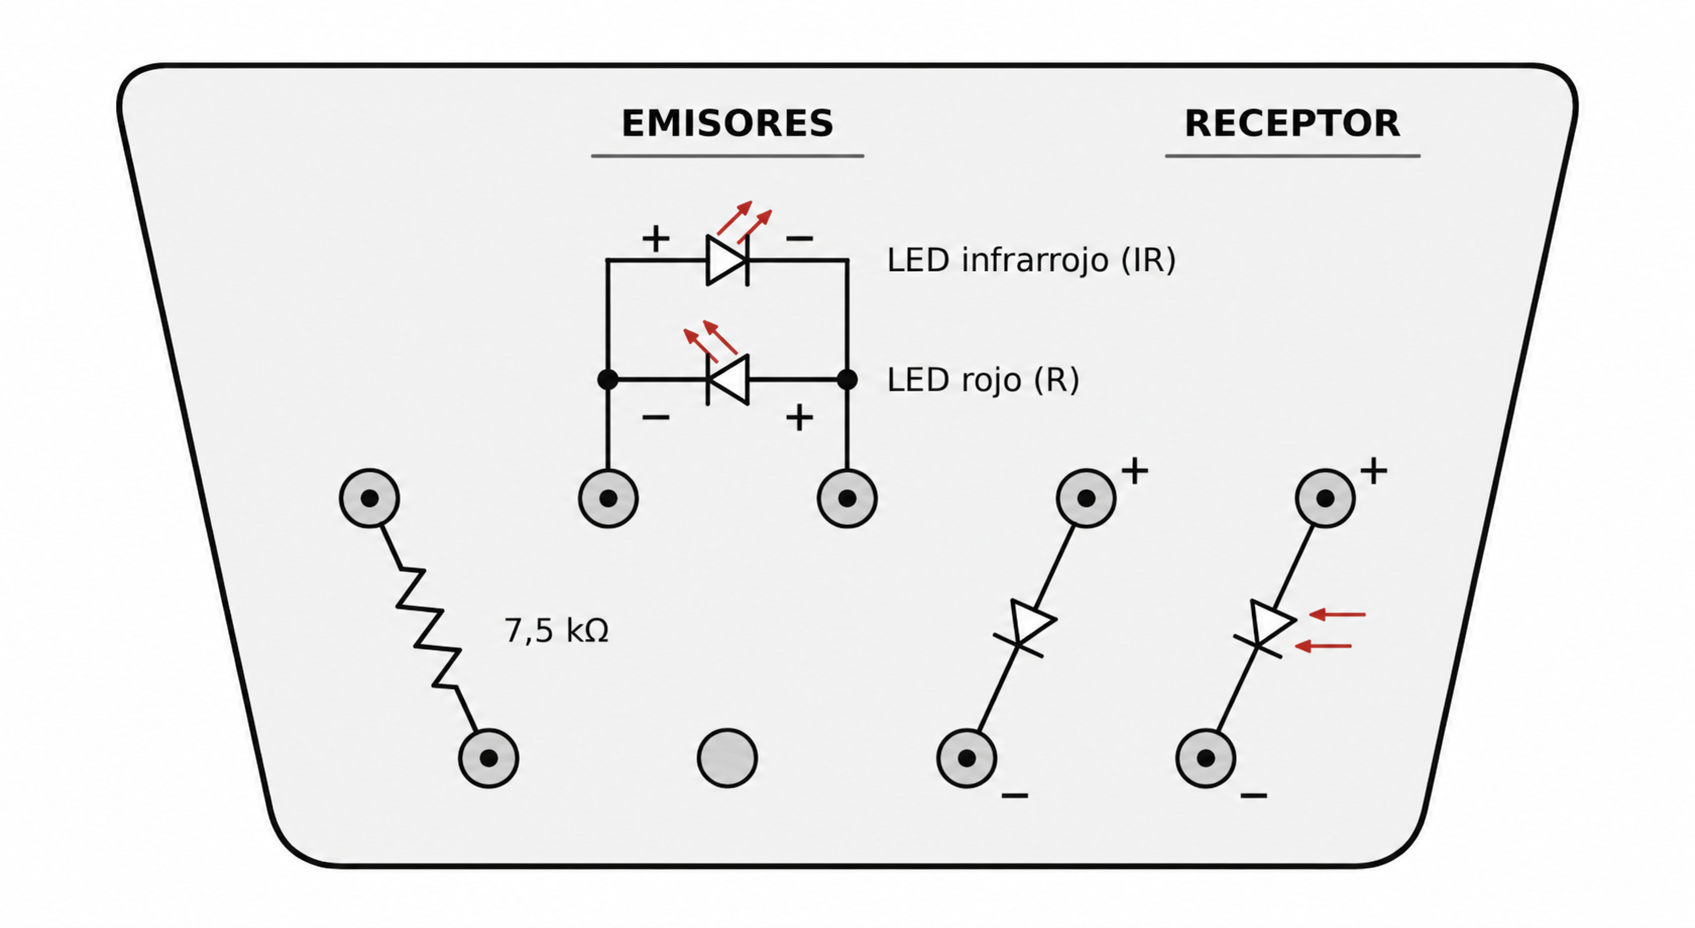
\includegraphics[width=0.85\textwidth]{Imagenes/D9.png}
    \caption{Distribución de los terminales y componentes internos del sensor Maicuff M2104-003A, identificados experimentalmente mediante un multímetro.}
    \label{fig:conexionado_sensor}
\end{figure}


\subsection{Implementación del circuito de adquisición}

Una vez identificados los terminales del sensor, se procedió al montaje en protoboard del circuito de adquisición pletismográfica propuesto en la consigna, respetando inicialmente los valores originales de sus componentes. El circuito está compuesto por una etapa de emisión y recepción óptica, seguida de etapas de filtrado y amplificación destinadas al acondicionamiento de la señal, como se muestra en la Figura~\ref{fig:circuito_original}.

\begin{figure}[H]
    \centering
    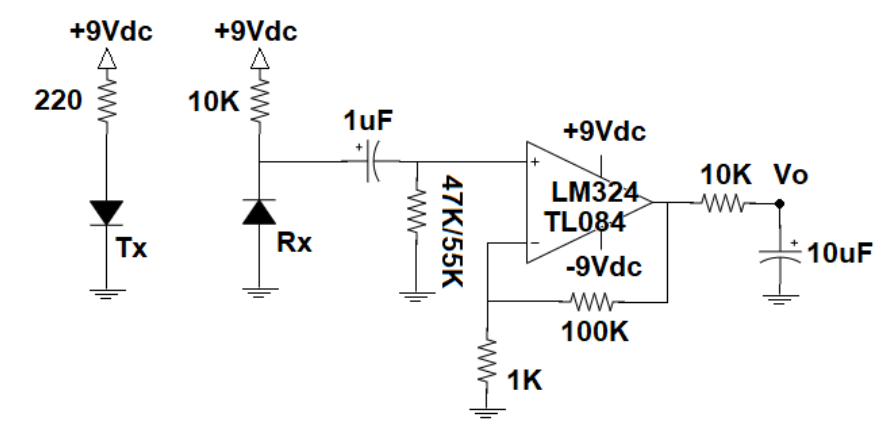
\includegraphics[width=0.9\textwidth]{Imagenes/Circuito.png}
    \caption{Circuito original de adquisición y acondicionamiento de la señal pletismográfica propuesto en la consigna.}
    \label{fig:circuito_original}
\end{figure}

En primer lugar, el LED rojo (Tx) se alimenta mediante una fuente de \SI{9}{\volt}, con una resistencia de \SI{220}{\ohm} en serie para limitar la corriente que circula por él. Por otro lado, el fotodetector (Rx) se conecta en polarización inversa, mediante una resistencia de \SI{10}{\kilo\ohm} vinculada a la alimentación de \SI{9}{\volt}. De esta manera, las variaciones de intensidad luminosa recibidas por el fotodetector producen cambios en la corriente que circula por él, los cuales se traducen en variaciones de tensión sobre la resistencia.

La señal obtenida pasa posteriormente por un capacitor de \SI{1}{\micro\farad} conectado en serie, junto con una resistencia de \SI{47}{\kilo\ohm} conectada a tierra. Estos componentes conforman un filtro pasa-altos de primer orden, cuya función es atenuar la componente continua y las variaciones de baja frecuencia de la señal.

La frecuencia de corte nominal de este filtro se determina mediante:

\begin{equation}
    f_{c,PA} = \frac{1}{2\pi RC}
    = \frac{1}{2\pi(47\times10^3)(1\times10^{-6})}
    \approx \SI{3.39}{\hertz}
\end{equation}

A continuación, la señal ingresa a un amplificador operacional, para el cual se utiliza un TL084, alimentado con tensiones de \SI{+9}{\volt} y \SI{-9}{\volt}. Este se encuentra configurado como amplificador no inversor, utilizando una resistencia de realimentación de \SI{100}{\kilo\ohm} y una resistencia de \SI{1}{\kilo\ohm} conectada a tierra. Por lo tanto, su ganancia teórica está dada por:

\begin{equation}
    A_v = 1 + \frac{R_f}{R_g}
    = 1 + \frac{100\,\text{k}\Omega}{1\,\text{k}\Omega}
    = 101
\end{equation}

Finalmente, a la salida del amplificador se incorpora una resistencia de \SI{10}{\kilo\ohm} en serie y un capacitor de \SI{10}{\micro\farad} conectado a tierra, formando un filtro pasa-bajos de primer orden. Esta etapa permite atenuar las componentes de mayor frecuencia presentes en la señal amplificada.

Su frecuencia de corte nominal se calcula mediante:

\begin{equation}
    f_{c,PB} = \frac{1}{2\pi RC}
    = \frac{1}{2\pi(10\times10^3)(10\times10^{-6})}
    \approx \SI{1.59}{\hertz}
\end{equation}

De esta manera, el circuito original permite transformar las variaciones de intensidad luminosa detectadas por el sensor en una señal de tensión amplificada y filtrada. Sin embargo, se observa que la frecuencia de corte del filtro pasa-altos es superior a la del pasa-bajos, lo que provoca una atenuación de las componentes de frecuencia intermedia y puede dificultar la adquisición de la señal pulsátil. Por lo tanto, resulta necesario analizar la selección de los componentes para mejorar la respuesta en frecuencia del sistema.


\subsection{Análisis y modificación de las etapas de filtrado}

A partir del análisis del circuito original, se observó que las frecuencias de corte de los filtros no resultaban adecuadas para la adquisición de la señal pletismográfica. En particular, el filtro pasa-altos presentaba una frecuencia de corte de \SI{3.39}{\hertz}, superior a la del filtro pasa-bajos, de \SI{1.59}{\hertz}. Esta configuración provocaba una atenuación considerable de las componentes de frecuencia asociadas a la actividad cardíaca.

Por este motivo, se propuso modificar los valores de los capacitores de ambas etapas, manteniendo las resistencias originales, con el objetivo de obtener una banda de paso más adecuada para la adquisición de la señal.

En primer lugar, para el filtro pasa-altos se reemplazó el capacitor de \SI{1}{\micro\farad} por uno de \SI{10}{\micro\farad}, manteniendo la resistencia de \SI{47}{\kilo\ohm}. De esta manera, la nueva frecuencia de corte nominal resulta:

\begin{equation}
    f_{c,PA} =
    \frac{1}{2\pi(47\times10^3)(10\times10^{-6})}
    \approx \SI{0.34}{\hertz}
\end{equation}

Esta modificación permite conservar las componentes de baja frecuencia correspondientes a las pulsaciones cardíacas, mientras se continúa atenuando la componente continua y las variaciones lentas de la línea de base.

Por otro lado, para el filtro pasa-bajos se reemplazó el capacitor de \SI{10}{\micro\farad} por uno de \SI{1}{\micro\farad}, manteniendo la resistencia de \SI{10}{\kilo\ohm}. La nueva frecuencia de corte nominal resulta:

\begin{equation}
    f_{c,PB} =
    \frac{1}{2\pi(10\times10^3)(1\times10^{-6})}
    \approx \SI{15.92}{\hertz}
\end{equation}

Con este cambio se busca conservar tanto la componente fundamental de la señal pletismográfica como sus armónicos, necesarios para representar adecuadamente la morfología de cada pulso, mientras se atenúan las componentes de mayor frecuencia.

En conjunto, las modificaciones realizadas permiten establecer una banda de paso nominal comprendida aproximadamente entre \SI{0.34}{\hertz} y \SI{15.92}{\hertz}, mejorando la respuesta en frecuencia del sistema respecto de la configuración original. De esta manera, se espera obtener una señal pletismográfica con menor atenuación de sus componentes de interés, facilitando su posterior visualización y análisis.

\section{Resultados}

\subsection{Resultados con la configuración original}

Al implementar el circuito con los valores originales de sus componentes, se logró visualizar una señal pletismográfica mediante el osciloscopio. Sin embargo, la señal obtenida presentaba una amplitud considerablemente reducida y una presencia de ruido que dificultaba su correcta visualización. A pesar de estas limitaciones, fue posible identificar las variaciones periódicas de la componente alterna, asociadas a los cambios de volumen sanguíneo producidos durante cada ciclo cardíaco, como se observa en la Figura~\ref{fig:curva_original}.

\begin{figure}[H]
    \centering
    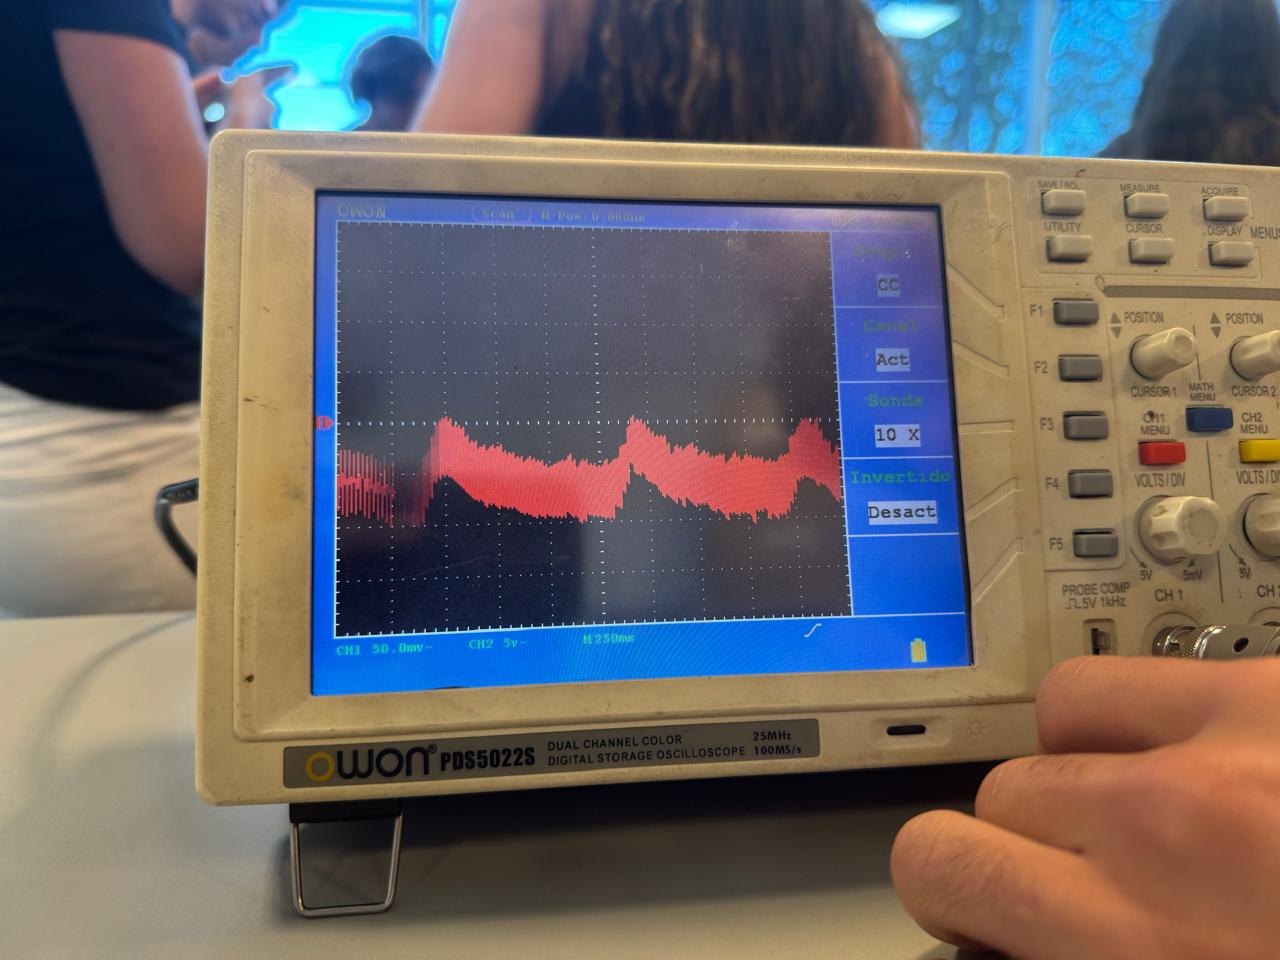
\includegraphics[width=0.85\textwidth]{Imagenes/CurvaOriginal.jpeg}
    \caption{Señal pletismográfica obtenida experimentalmente mediante el osciloscopio, utilizando la configuración original del circuito.}
    \label{fig:curva_original}
\end{figure}

Estas dificultades podrían atribuirse principalmente a la selección de las frecuencias de corte de los filtros y a las características de la etapa de amplificación. Como se analizó anteriormente, el filtro pasa-altos presentaba una frecuencia de corte de \SI{3.39}{\hertz}, mientras que la del pasa-bajos era de \SI{1.59}{\hertz}, provocando una atenuación considerable de las componentes de interés. Asimismo, aunque el amplificador presentaba una ganancia teórica de 101, esta no necesariamente resultaba suficiente para compensar la baja amplitud de la señal adquirida y las pérdidas introducidas por el filtrado.

Por lo tanto, si bien el circuito permitió detectar la actividad pulsátil, los resultados obtenidos evidenciaron la necesidad de modificar las etapas de filtrado para mejorar la amplitud y facilitar la identificación de la señal pletismográfica.

\section{Conclusiones}

La implementación del circuito permitió adquirir y visualizar una señal pletismográfica, identificando las variaciones periódicas asociadas a la actividad cardíaca. Sin embargo, la reducida amplitud y la presencia de ruido dificultaron su visualización, evidenciando limitaciones en el acondicionamiento de la señal.

A partir del análisis teórico posterior a la práctica, se identificó que las frecuencias de corte originales de los filtros provocaban una atenuación considerable de las componentes de interés. Por este motivo, se propusieron modificaciones en los valores de los capacitores para mejorar la respuesta en frecuencia del sistema.

En conclusión, el trabajo permitió comprender la importancia de una correcta selección de las etapas de filtrado y amplificación. Si bien las modificaciones propuestas no fueron implementadas experimentalmente, su análisis permitió identificar posibles mejoras para obtener una señal pletismográfica de mayor amplitud y calidad.


\end{document}
